\section{Vorbereitende Aufgaben}
    \subsection{Kürzester Burgers Vektor in LiF}
        Da es sich bei LiF um eine FCC-Gitterstruktur handelt, ist der nächste gleichartiger Kern stehts an Position $\frac{1}{2} * <110>$. Daraus folgt für unseren minimalen
        Burgers Vektor eine Länge von
        \begin{align}
            |<110>| = a \cdot \sqrt{2} \\
            \frac{1}{2} \cdot \frac{a}{\sqrt{2}} = \frac{a}{\sqrt{2}}
        \end{align}
        Längere Burgers Vektoren sind daher sehr unwahrscheinlich, da die aufzuwendende Energie für eine Verschiebung sich $\propto |\vec{b}|^2$ Verhält.
    \subsection{Abstand d zwischen zwei Ätzgrübchen}
        $a = 0.402nm$
        \begin{equation}
            \theta = \arctan{\frac{b}{d}} = \arctan{\frac{a}{d \sqrt{2}}}
        \end{equation}
    \subsection{Versetzungen durch Nadeleindruck}
        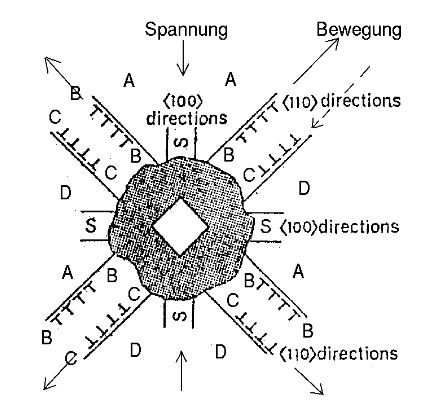
\includegraphics{Images/Question3.PNG}
    \subsection{1234}
        \hl{Unterschied zwischen Axialem Druck und Nadeleindruck}